% Section content template for individual Educative lessons
% This file contains the actual content for a specific section
% Generated from Educative API section content

% Section: Class Diagram for the Parking Lot
% Section ID: 6722059256463360
% Section Slug: class-diagram-for-the-parking-lot
% Generated: 2025-12-11T13:40:18.872946

In this lesson, we will identify, design, and explain the classes and abstract classes and their relationships that form the backbone of our parking lot system. We 'll use SOLID principles, extensibility, and object-oriented design best practices.

\subsection{Components of a parking lot system}\label{3U1e8cD3M4xGVCXTeJbJ1}
\\
As our requirements outline, the system involves various entities and their interactions. We will use a bottom-up approach:

\begin{itemize}
\item
\protect\phantomsection\label{ruKsU6jrcWBIyY8UjIF94}
First, design the smallest, most fundamental entities.
\item
\protect\phantomsection\label{Go0Gqn6TX_npG1adTj9tp}
Next, combine these to form more complex system components.
\item
\protect\phantomsection\label{vZY2IExRQNQXtMmPVV6Kq}
Finally, bring everything together in the main \texttt{ParkingLot} class, responsible for coordination.
\end{itemize}

\subsubsection{Vehicle}\label{PBFiZdprecXihr7jm9hSC}
\\
Our parking lot system should have a vehicle object according to the requirements. The vehicle can be a car, a truck, a van, or a motorcycle. There are two ways to represent a vehicle in our system:

\begin{itemize}
\item
\protect\phantomsection\label{737wfNLXKdkJp6YE5g5m2}
Enumeration
\item
\protect\phantomsection\label{xud_hjjAi1QZcDZtGA_lU}
Abstract class
\end{itemize}
\\
\paragraph{Enumeration vs. abstract class}\label{vHDzvtFbMHcpb8o5oqkld}
\\
Theenumeration class creates a user-defined data type with the four vehicle types as values.
\\
This approach is not proficient for object-oriented design because if we want to add one more vehicle type later in our system, we need to update the code in multiple places, violating the Open/Closed principle of the SOLID design principles. The Open/Closed principle states that classes can be extended but not modified. Therefore, it is recommended not to use the enumeration data type as it is not a scalable approach.
\begin{quote}
\textbf{Note:} Using enums isn't prohibited, but it is not recommended. Later, we will use the \texttt{PaymentStatus} enum in our parking lot design, as it won't require further modifications.
\end{quote}
\\
An abstract class cannot instantiate an object and can only be used as a base class. The abstract class for \texttt{Vehicle} is the best approach. It allows us to create derived child classes for the \texttt{Vehicle} class. It can also be extended easily in case the vehicle type changes.

\begin{figure}[htbp]
 \centering
 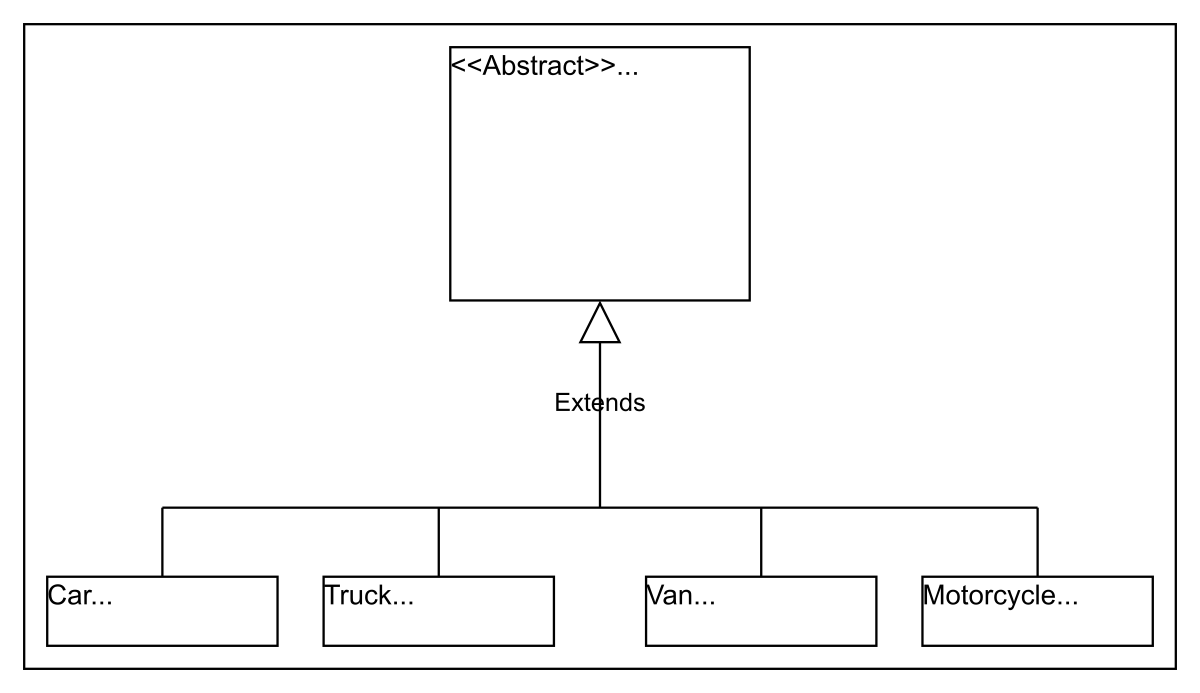
\includegraphics[width=0.5\textwidth]{Images/chapter_7/section_6722059256463360/6071383044784128.png}
 \caption{The class diagram of Vehicle and its derived classes}
\end{figure}

\textbf{R1:} The parking lot must support a total capacity of up to 40,000 vehicles.
\\
\textbf{R4:} The system must support parking for four types of vehicles: cars, trucks, vans, and motorcycles.
\\
\textbf{R6:} The system must not allow more vehicles to enter once the parking lot reaches its maximum capacity.
\\
\textbf{R10:} The parking lot system must support configurable pricing rates based on vehicle type and/or parking spot type and different rates for different parking durations (e.g., first hour, subsequent hours).

\subsubsection{Parking spot}\label{VB-a0gzbl1Vlz8sozqCrS-1}
\\
Similar to the \texttt{Vehicle} class, the \texttt{ParkingSpot} should also be an abstract class. There are four parking spots: accessible, compact, large, and motorcycle. These classes can be derived from the parking spot abstract class.

\begin{figure}[htbp]
 \centering
 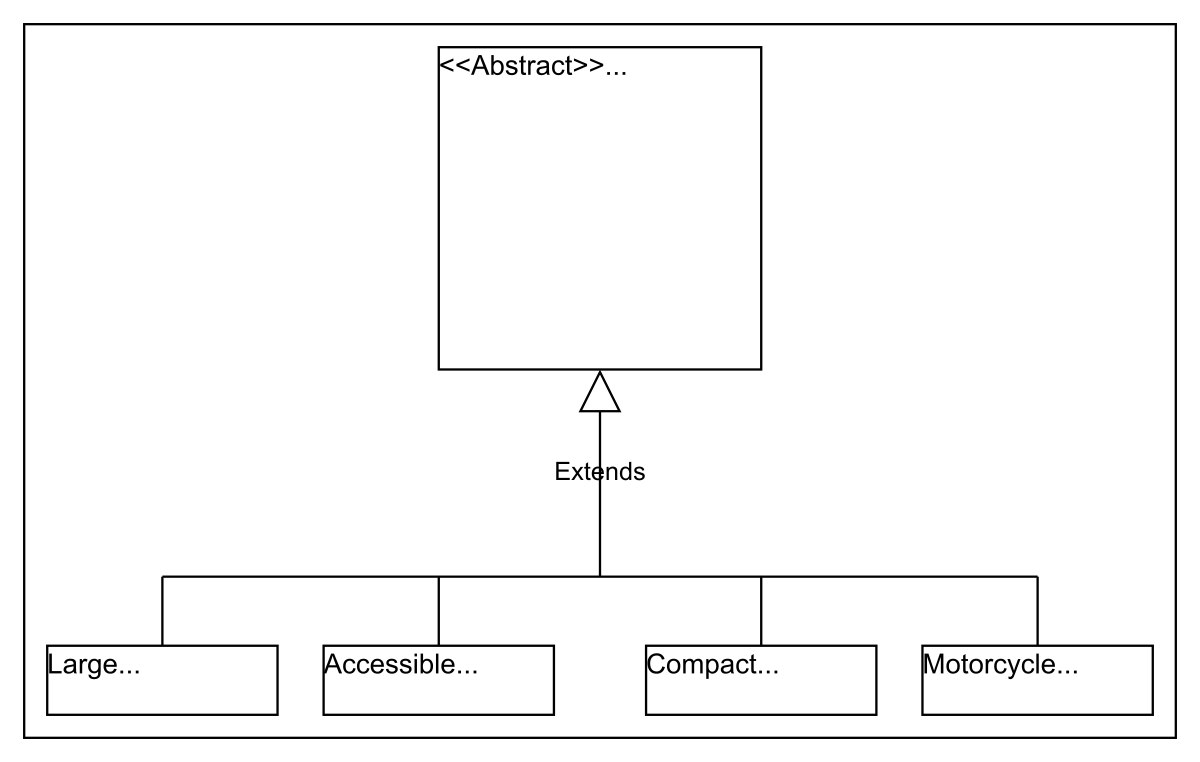
\includegraphics[width=0.5\textwidth]{Images/chapter_7/section_6722059256463360/5131329103331328.png}
 \caption{The class diagram of the ParkingSpot and its derived classes}
\end{figure}

\textbf{R1:} The parking lot must support a total capacity of up to 40,000 vehicles.
\\
\textbf{R2:} The parking lot must support multiple types of parking spots:

\begin{itemize}
\tightlist
\item
Accessible
\item
Compact
\item
Large
\item
Motorcycle
\end{itemize}
\\
\textbf{R5:} A display board at each entrance and on every floor should show the current available parking spots for each parking spot type.
\\
\textbf{R6:} The system must not allow more vehicles to enter once the parking lot reaches its maximum capacity.
\\
\textbf{R7:} When the parking lot is fully occupied, a clear message should be displayed at each entrance and on all parking lot display boards.

\subsubsection{Account}\label{T7Dldmr7BJxwBTnuPS_y2}
\\
Like to the~\texttt{Vehicle}~and~\texttt{ParkingSpot}~classes,~\texttt{Account}~should also be an abstract class. The ~\texttt{Admin}~class is derived from this abstract class.

\begin{figure}[htbp]
 \centering
 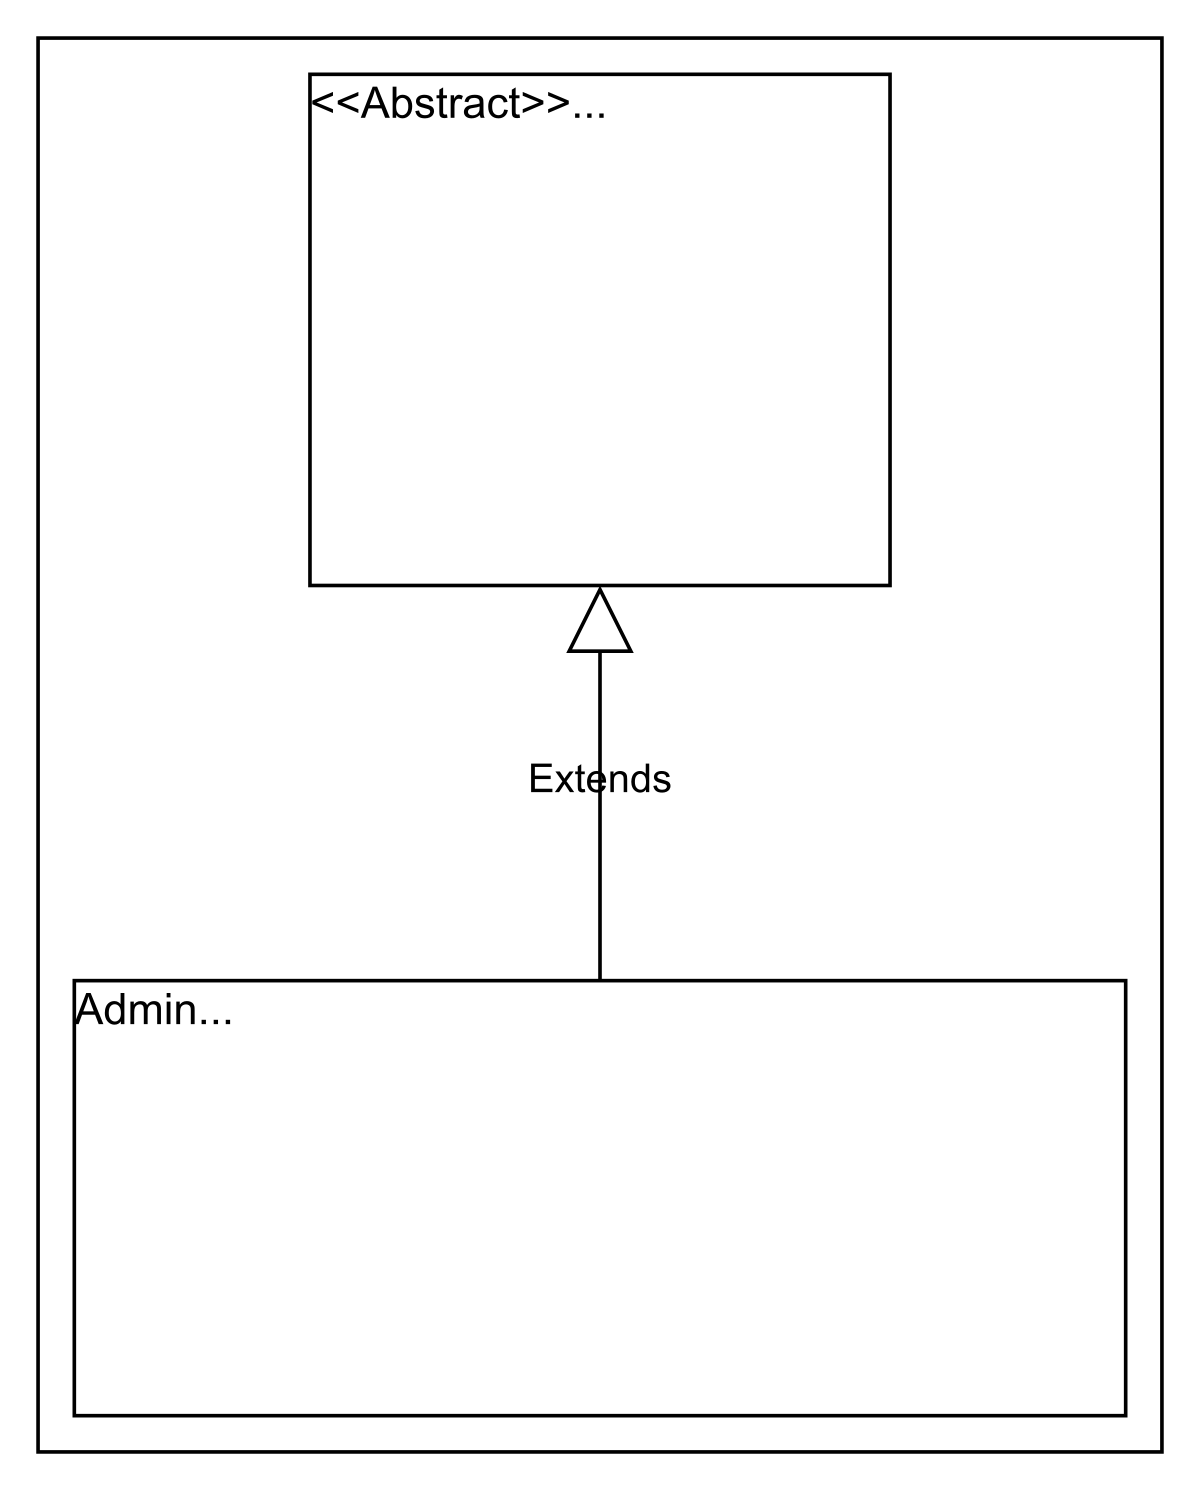
\includegraphics[width=0.5\textwidth]{Images/chapter_7/section_6722059256463360/5779297418477568.png}
 \caption{The class diagram of Account and its derived classes}
\end{figure}

\textbf{R2:} The parking lot must support multiple types of parking spots:

\begin{itemize}
\tightlist
\item
Accessible
\item
Compact
\item
Large
\item
Motorcycle
\end{itemize}
\\
\textbf{R3:} The parking lot should provide multiple entrance and exit points to support efficient traffic flow.
\\
\textbf{R5:} A display board at each entrance and on every floor should show the current available parking spots for each parking spot type.
\\
\textbf{R10:} The parking lot system must support configurable pricing rates based on vehicle type and/or parking spot type and different rates for different parking durations (e.g., first hour, subsequent hours).

\subsubsection{Display board}\label{VB-a0gzbl1Vlz8sozqCrS-2}
\\
This class represents the free parking spot types and the number of empty slots.

\begin{figure}[htbp]
 \centering
 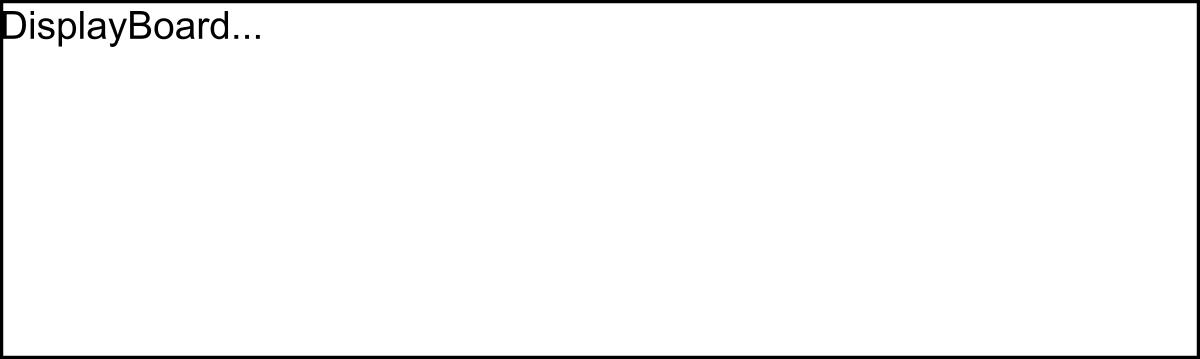
\includegraphics[width=0.5\textwidth]{Images/chapter_7/section_6722059256463360/6346733045022720.png}
 \caption{The class diagram of the DisplayBoard class}
\end{figure}

\textbf{R5:} A display board at each entrance and on every floor should show the current available parking spots for each parking spot type.
\\
\textbf{R7:} When the parking lot is fully occupied, a clear message should be displayed at each entrance and on all parking lot display boards.

\subsubsection{Entrance and exit}\label{VB-a0gzbl1Vlz8sozqCrS-3}
\\
The \texttt{Entrance} class generates the parking ticket whenever a vehicle arrives. There are multiple entrances to the parking lot, so it contains the ID attribute and has the \texttt{getTicket()} method.
\\
The \texttt{Exit} class is responsible for validating the parking ticket's payment status before allowing the vehicle to exit the parking lot. As there are multiple exits to the parking lot, it contains the ID attribute and has the \texttt{validateTicket()} method.

\begin{figure}[htbp]
 \centering
 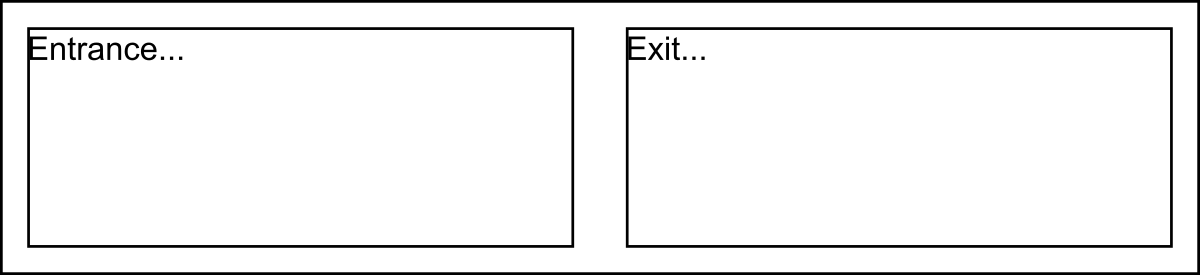
\includegraphics[width=0.5\textwidth]{Images/chapter_7/section_6722059256463360/5192259303899136.png}
 \caption{The class diagram of the Entrance and Exit classes}
\end{figure}

\textbf{R3:} The parking lot should provide multiple entrance and exit points to support efficient traffic flow.
\\
\textbf{R8:} Customers must be issued a parking ticket at entry. The ticket will be used to track parking time and calculate payment at exit.
\\
\textbf{R9:} Customers should be able to pay for parking at the automated exit panel.

\subsubsection{Parking ticket}\label{VB-a0gzbl1Vlz8sozqCrS-4}
\\
The \texttt{ParkingTicket} class is one of the system's central classes. It tracks the vehicles' entrance and exit times, the amount, and the payment status.

\begin{figure}[htbp]
 \centering
 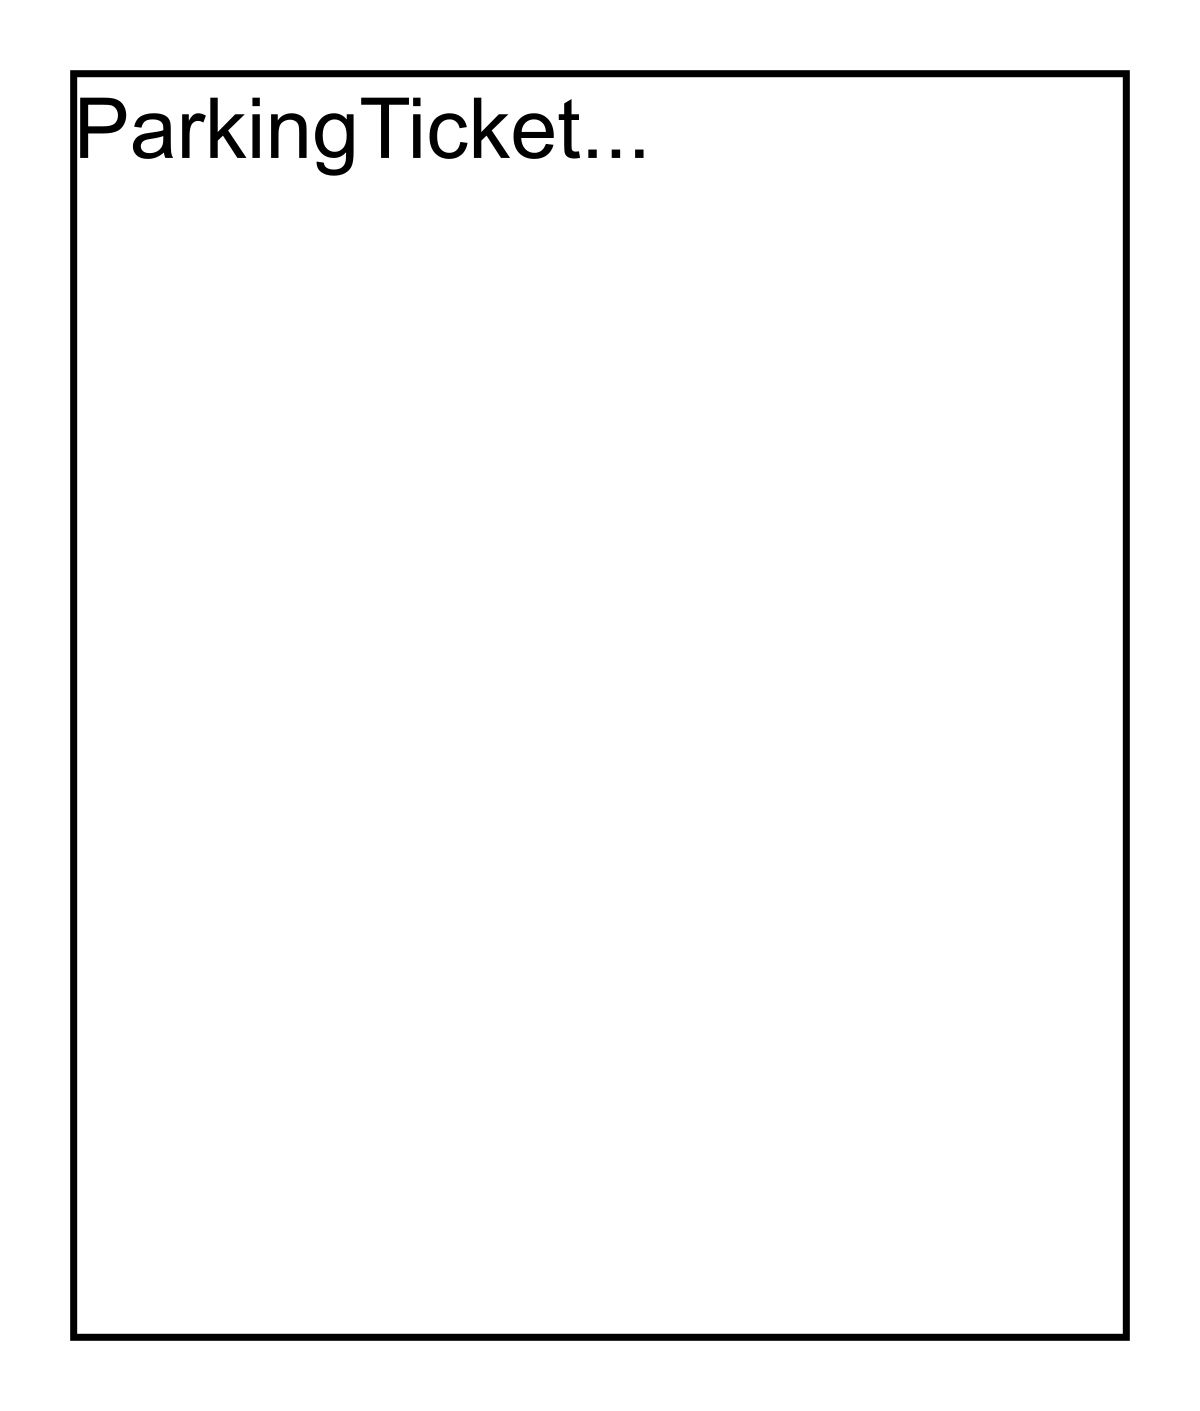
\includegraphics[width=0.5\textwidth]{Images/chapter_7/section_6722059256463360/5928409111592960.png}
 \caption{The class diagram of the ParkingTicket class}
\end{figure}

\textbf{R8:} Customers must be issued a parking ticket at entry. The ticket will be used to track parking time and calculate payment at exit.
\\
\textbf{R10:} The parking lot system must support configurable pricing rates based on vehicle type and/or parking spot type and different rates for different parking durations (e.g., first hour, subsequent hours).

\subsubsection{Payment}\label{VB-a0gzbl1Vlz8sozqCrS-5}
\\
The \texttt{Payment} class will be abstract and have two child classes, \texttt{CreditCard} and \texttt{Cash}, as these are the two payment methods in the parking lot system.

\begin{figure}[htbp]
 \centering
 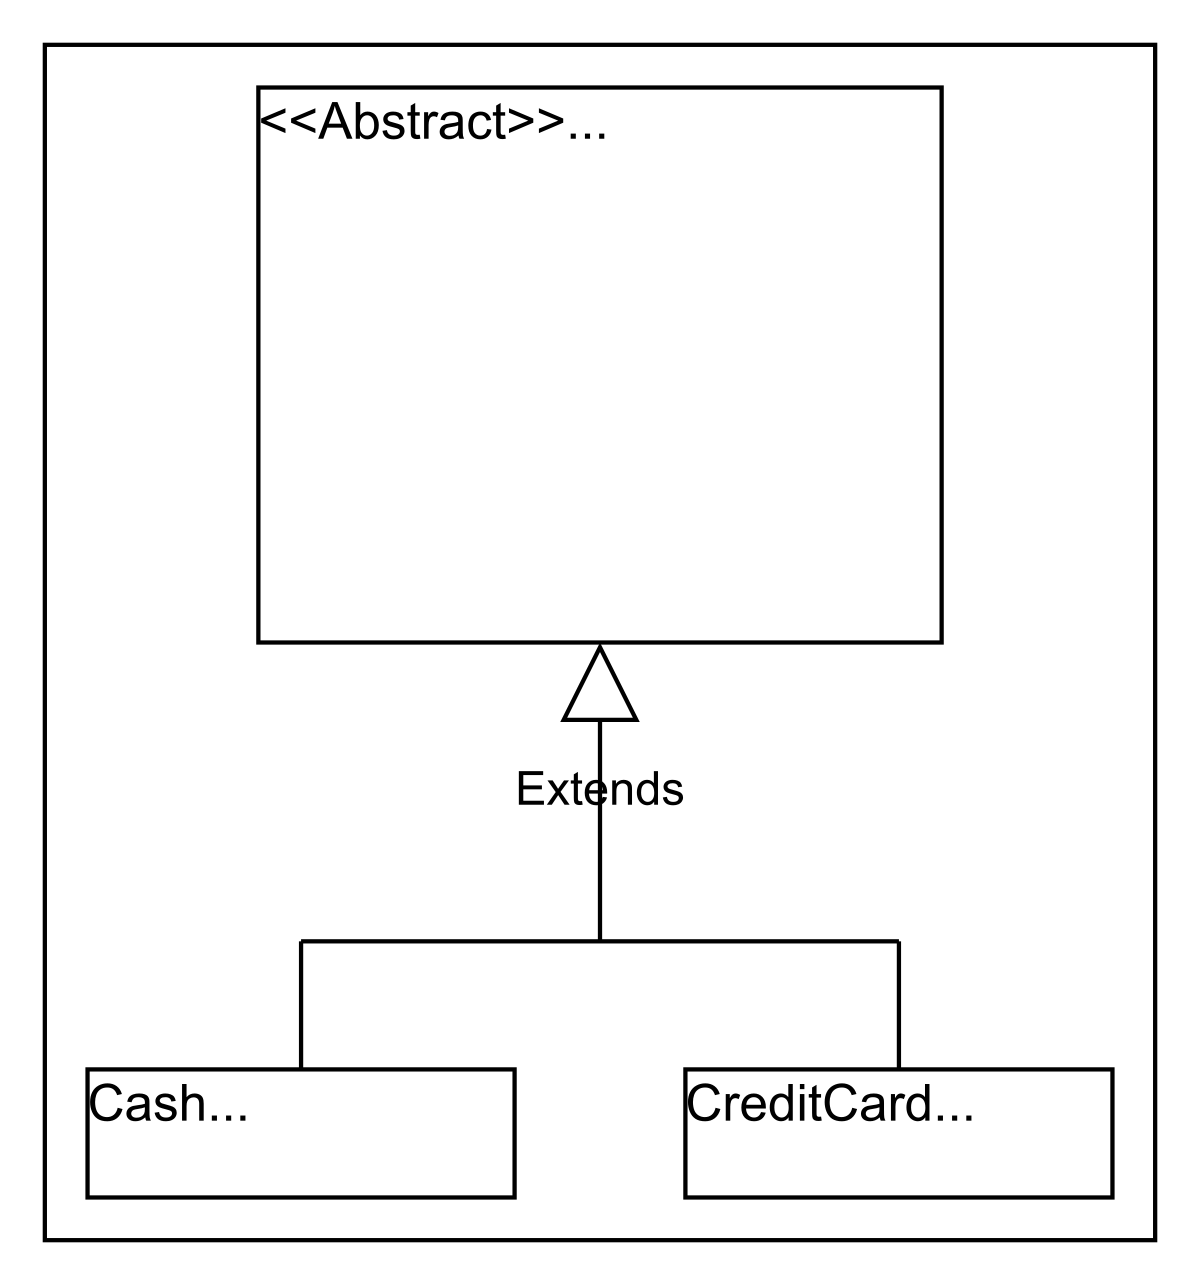
\includegraphics[width=0.5\textwidth]{Images/chapter_7/section_6722059256463360/4783287254777856.png}
 \caption{The class diagram of the Payment class}
\end{figure}

\textbf{R9:} Customers should be able to pay for parking at the automated exit panel.
\\
\textbf{R10:} The parking lot system must support configurable pricing rates based on vehicle type and/or parking spot type and different rates for different parking durations (e.g., first hour, subsequent hours).
\\
\textbf{R11:} Payments must be accepted via credit/debit card and cash at all payment points.

\subsubsection{Parking rate}\label{VB-a0gzbl1Vlz8sozqCrS-6}
\\
The \texttt{ParkingRate} class is responsible for calculating the final payment based on the time spent in the parking lot.

\begin{figure}[htbp]
 \centering
 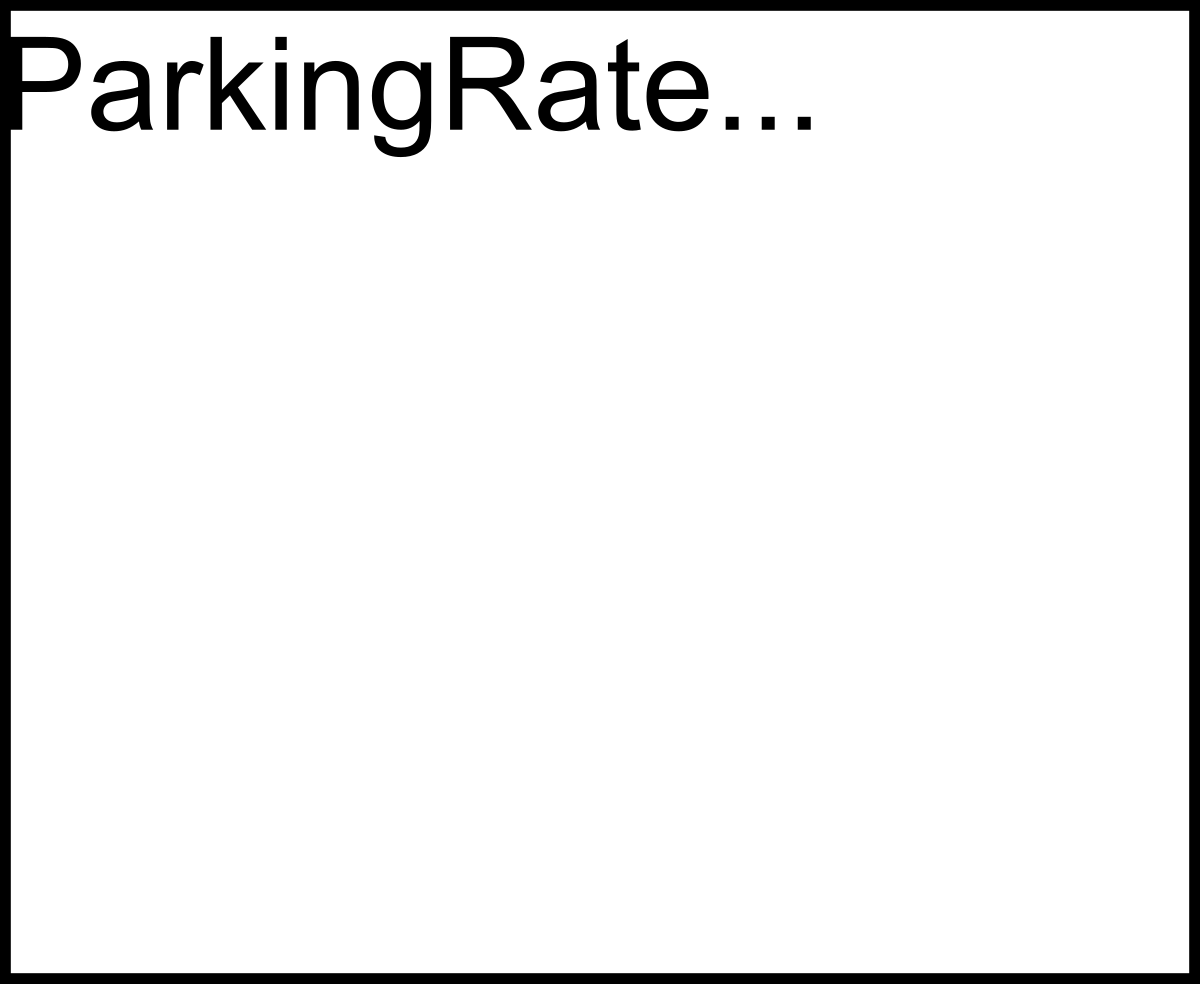
\includegraphics[width=0.5\textwidth]{Images/chapter_7/section_6722059256463360/4589781033156608.png}
 \caption{The class diagram of the ParkingRate class}
\end{figure}

\textbf{R10:} The parking lot system must support configurable pricing rates based on vehicle type and/or parking spot type, as well as different rates for different parking durations (e.g., first hour, subsequent hours).

\subsubsection{Parking lot}\label{VB-a0gzbl1Vlz8sozqCrS-7}
\\
Now, we will discuss the design of the whole \texttt{ParkingLot} system class. This parking lot system comprises smaller objects we have already designed, like entrance/exit, parking spots, parking rates, etc.

\begin{figure}[htbp]
 \centering
 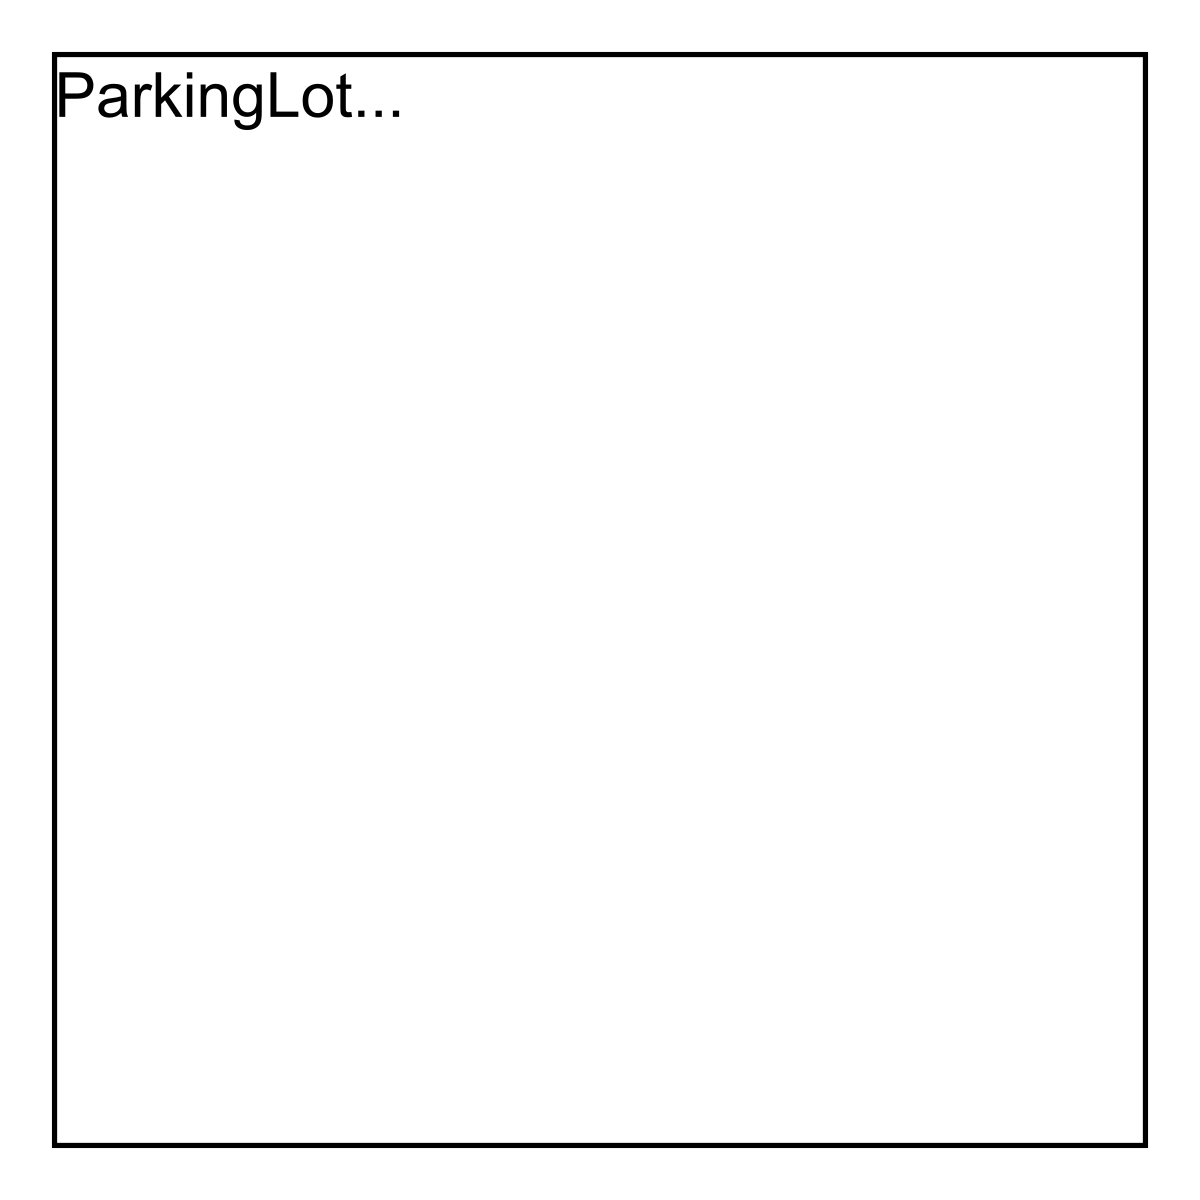
\includegraphics[width=0.5\textwidth]{Images/chapter_7/section_6722059256463360/4664255725830144.png}
 \caption{The class diagram for the ParkingLot class}
\end{figure}

\subsubsection{The enumerations and custom data types}\label{lTqA4q4Rq1gELYLeamRjz-1}
\\
The following provides an overview of the enumerations and custom data types used in this problem:

\begin{itemize}
\item
\texttt{PaymentStatus}\textbf{:} We need to create an enumeration to keep track of the parking ticket's payment status, such as whether it is paid, unpaid, canceled, refunded, and so on.
\item
\texttt{AccountStatus}\textbf{:} We need to create an enumeration to keep track of the status of the account, whether it is active, canceled, closed, and so on.
\item
\protect\phantomsection\label{xYnlSAzNijrYMcy4wkE5O}
\texttt{TicketStatus}\textbf{:} We need to create an enumeration to track the current status of a parking ticket, such as whether it is issued, in use, paid, validated, canceled, refunded, and so on.
\end{itemize}

\begin{figure}[htbp]
 \centering
 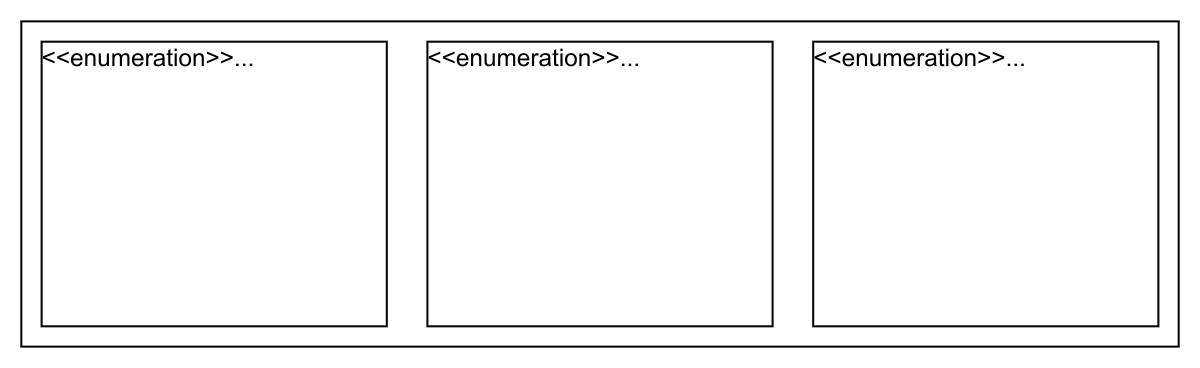
\includegraphics[width=0.5\textwidth]{Images/chapter_7/section_6722059256463360/4999235324739584.png}
 \caption{Enums in the parking lot system}
\end{figure}

\paragraph{Address}\label{lTqA4q4Rq1gELYLeamRjz-2}
\\
We also need to create a custom data type, \texttt{Address}, to store the parking lot\textquotesingle s location.

\begin{figure}[htbp]
 \centering
 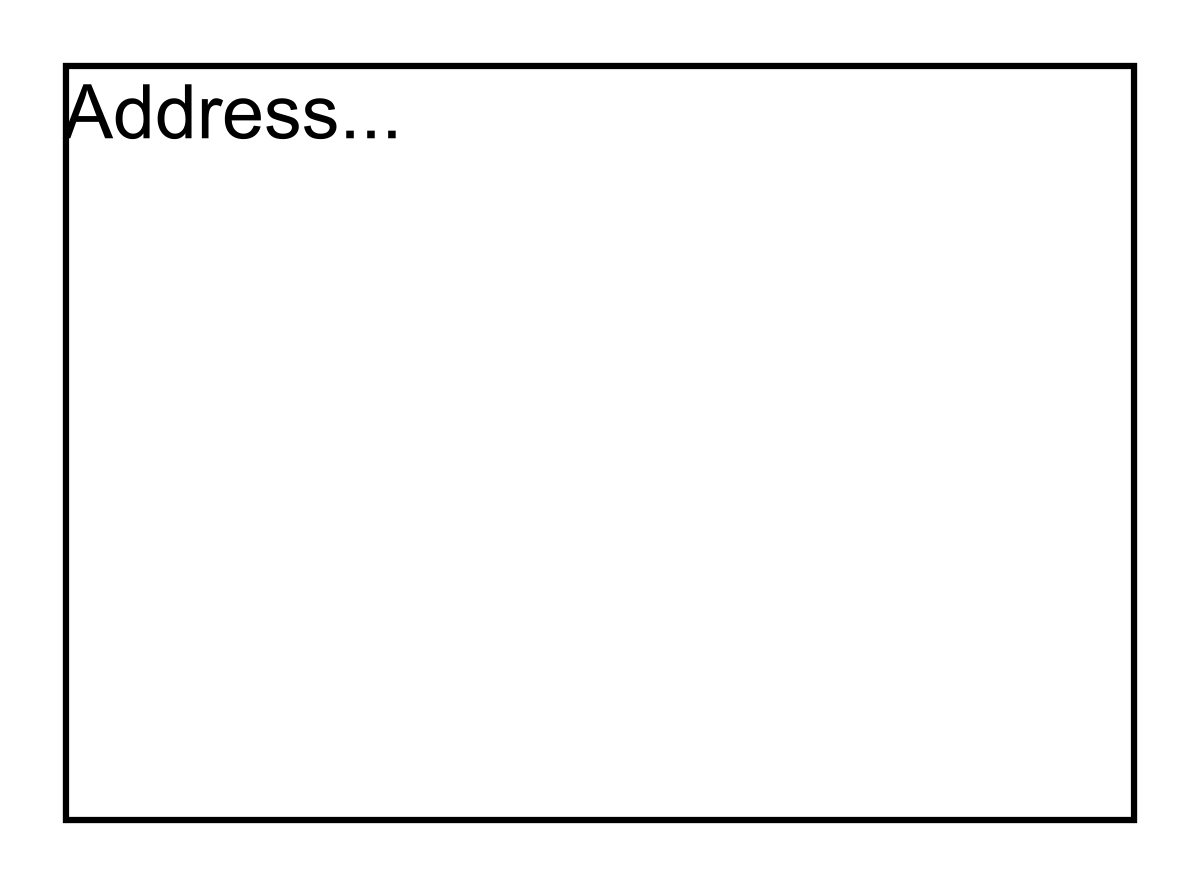
\includegraphics[width=0.5\textwidth]{Images/chapter_7/section_6722059256463360/5625086405902336.png}
 \caption{The class diagram of the Address custom data type}
\end{figure}

\subsubsection{Person}\label{_uE63ZRiaToKjqqTZvARE}
\\
The \texttt{Person} class stores information related to a person, such as their name, street address, country, etc.

\begin{figure}[htbp]
 \centering
 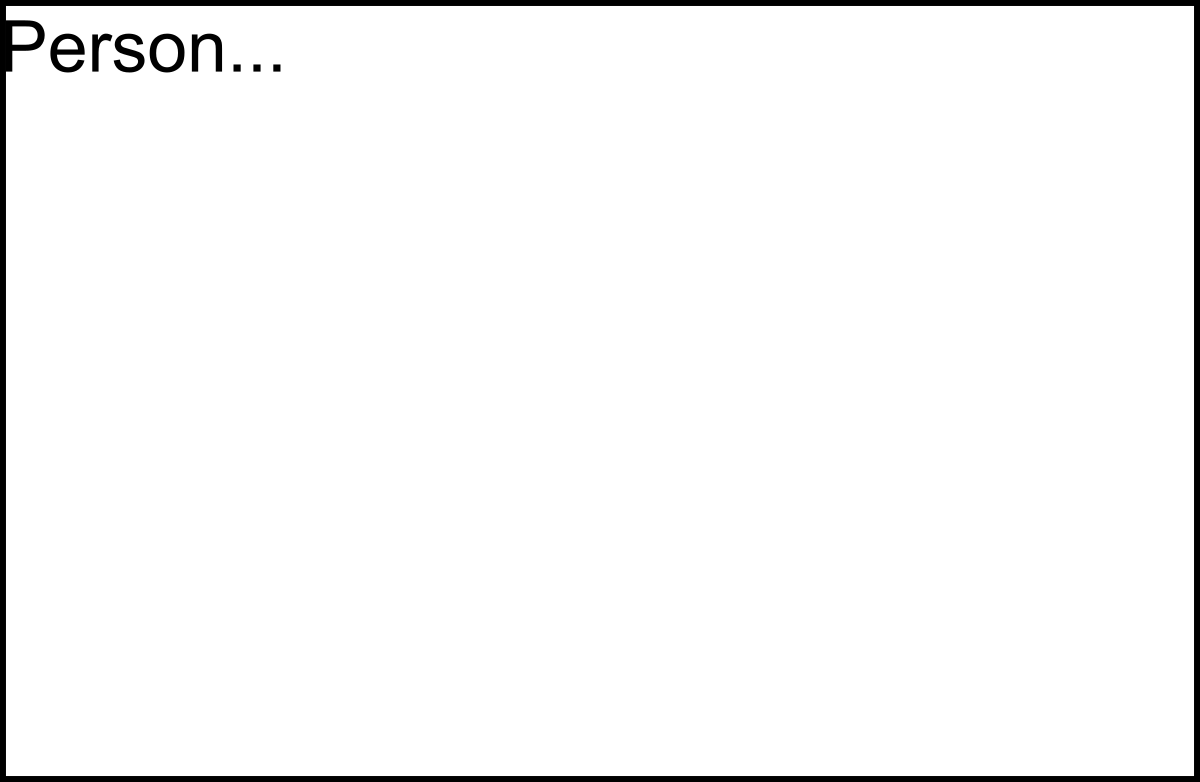
\includegraphics[width=0.5\textwidth]{Images/chapter_7/section_6722059256463360/5235199950716928.png}
 \caption{The class diagram of the Person class custom data type}
\end{figure}

\subsection{Relationship between the classes}\label{lTqA4q4Rq1gELYLeamRjz-3}
\\
Now, we'll discuss the relationships between the classes we have defined above in our parking lot system.

\subsubsection{Association}\label{CZzEgZfT0fr9TOIbG4X2y}
\\
An association represents a \emph{loose relationship} between two classes, where one class refers to another to use its functionality or store a reference. Associations typically do not imply ownership, and the associated object may exist independently of the referring object.
\\
In the parking lot system, association relationships include:

\begin{itemize}
\item
\protect\phantomsection\label{IRLozvYlUHbxxaNVVlkZO}
Each \texttt{ParkingSpot} is associated with a \texttt{Vehicle} object. When a vehicle is parked, the spot keeps a reference to the vehicle. This allows the parking spot to track which vehicle is currently occupying it. However, the vehicle does not directly reference its spot.
\item
\protect\phantomsection\label{c5ulMa-TgWqgqLA8WJK70}
A \texttt{Vehicle} is associated with its current \texttt{ParkingTicket}. When a vehicle enters the lot, it receives a ticket, which allows for tracking and processing of parking sessions.
\item
\protect\phantomsection\label{9hsmfXnAZW5T2PQdFU7br}
The \texttt{ParkingTicket} class maintains references to the \texttt{Entrance}, \texttt{Exit}, and \texttt{Vehicle} involved in the parking session, allowing the system to trace the entry and exit points and the vehicle details for any given ticket.
\item
\protect\phantomsection\label{kzwReCB19KzLGwqz91XhT}
The \texttt{DisplayBoard} and \texttt{ParkingSpot} should have an association relationship. The
\texttt{DisplayBoard} is responsible for showing the availability/status of multiple \texttt{ParkingSpot} objects; it maintains a reference (typically a list or map) to all spots it displays.
\end{itemize}

\begin{figure}[htbp]
 \centering
 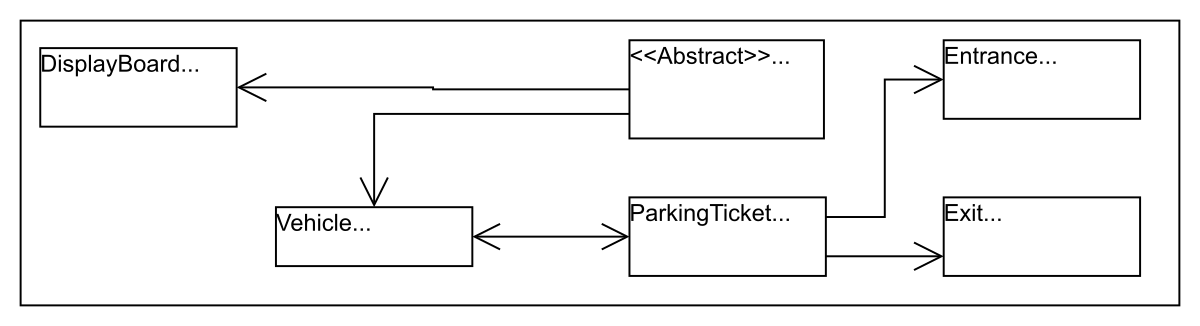
\includegraphics[width=0.5\textwidth]{Images/chapter_7/section_6722059256463360/5074138765852672.png}
 \caption{The association relationship between classes}
\end{figure}

\subsubsection{Composition}\label{9XjrLNsN2G8N1t7BivR_q}
\\
Composition is a \emph{strong form} of association that implies ownership and a whole-part relationship. When a composite object is destroyed, its components are destroyed as well. In other words, the composed objects do not exist independently of their parent.
\\
In our parking lot system, composition relationships are seen in:

\begin{itemize}
\item
The \texttt{ParkingLot} class comprises its key components, including all instances of \texttt{Entrance}, \texttt{Exit}, \texttt{ParkingSpot}, \texttt{DisplayBoard}, \texttt{ParkingRate}, and all current \texttt{ParkingTicket} objects. The parking lot is responsible for creating, managing, and destroying these components, which do not exist outside the context of the parking lot.
\item
\protect\phantomsection\label{YlHZyfBN68egBLOABXdZS}
Each \texttt{ParkingTicket} is composed of a \texttt{Payment} object. The payment represents the financial transaction for that specific parking session and is created and managed by the ticket; it does not exist independently outside the ticket.
\end{itemize}

\begin{figure}[htbp]
 \centering
 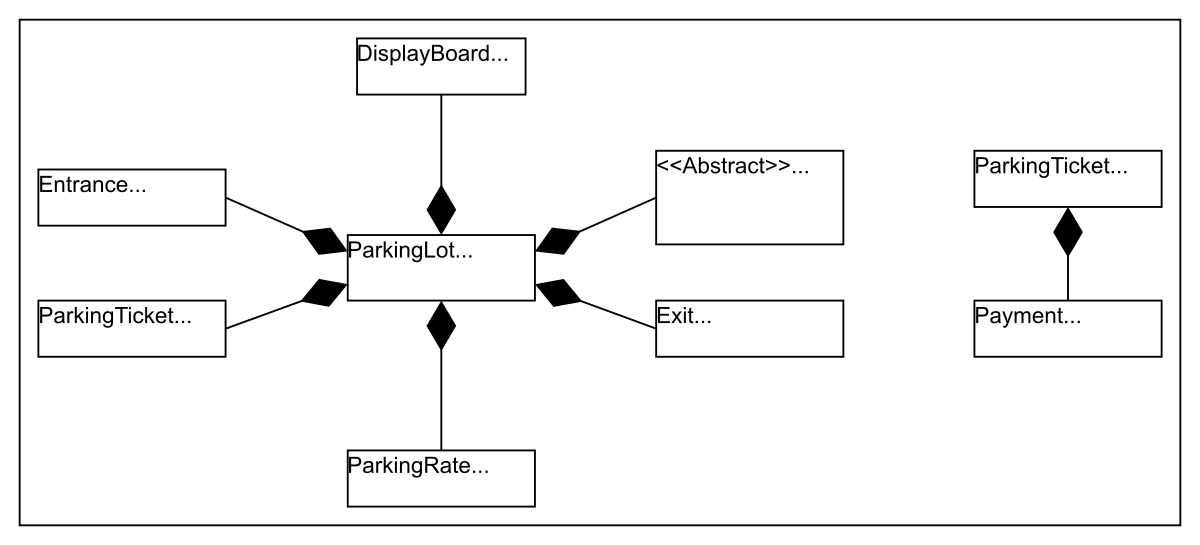
\includegraphics[width=0.5\textwidth]{Images/chapter_7/section_6722059256463360/6201344418250752.png}
 \caption{The composition relationship between classes}
\end{figure}

\subsubsection{Inheritance}\label{VB-a0gzbl1Vlz8sozqCrS-8}
\\
Inheritance, or generalization, is a relationship in which one class (the child or subclass) inherits behavior and attributes from another class (the parent or superclass). This allows for code reuse and logical grouping of shared functionality while enabling polymorphic behavior.
\\
In the parking lot system, inheritance relationships are structured as follows:

\begin{itemize}
\item
\protect\phantomsection\label{GkBJdiiaKDXMwOSglpxj4}
The abstract \texttt{Vehicle} class serves as the general blueprint for different types of vehicles, with \texttt{Car}, \texttt{Truck}, \texttt{Van}, and \texttt{Motorcycle} as its concrete subclasses. Each subclass can extend or override the behavior defined in \texttt{Vehicle}.
\item
Similarly, the abstract \texttt{ParkingSpot} class defines a parking spot's core properties and behaviors. The specific spot types---\texttt{AccessibleSpot}, \texttt{CompactSpot}, \texttt{LargeSpot}, and \texttt{MotorcycleSpot}---are implemented as subclasses, each potentially providing specialized logic for assigning vehicles.
\item
\protect\phantomsection\label{mfoqeZiA_IfKBoEmCATwn}
The \texttt{Payment} abstract class provides the basic structure for payment operations, while \texttt{Cash} and \texttt{CreditCard} classes implement the details for each payment method.
\end{itemize}
\begin{quote}
\textbf{Note:} The component section above has already discussed the inheritance relationship between classes.
\end{quote}
\subsection{Class diagram of the parking lot system}\label{R5gtrTOfMYj7zxHvFk9-u}
\\
This section outlines the multiplicity (cardinality) relationships between the main classes in our parking lot system. We explain the allowed number of instances on each side for each relationship and the real-world or design rationale behind the connection. Understanding these relationships is key to modeling how different entities interact and collaborate to support key workflows in the system.

\begin{center}
\renewcommand{\arraystretch}{1.4}

\begin{longtable}{|p{0.18\linewidth}|p{0.18\linewidth}|p{0.18\linewidth}|p{0.36\linewidth}|}
\hline
\textbf{Source} & \textbf{Target} & \textbf{Multiplicity} & \textbf{Reason} \\
\hline
\endfirsthead

\hline
\textbf{Source} & \textbf{Target} & \textbf{Multiplicity} & \textbf{Reason} \\
\hline
\endhead

\hline
\endfoot

\hline
\endlastfoot

ParkingLot & Entrance & 1 -- 1..* & A parking lot must have at least one entrance, and can have multiple for efficient flow. \\
\hline
ParkingLot & Exit & 1 -- 1..* & A parking lot must have at least one exit, and can have multiple for smooth operation. \\
\hline
ParkingLot & ParkingSpot & 1 -- 1..* & Every parking lot manages multiple parking spots. \\
\hline
ParkingLot & ParkingTicket & 1 -- 0..* & The lot manages zero or more tickets at any given time. \\
\hline
ParkingLot & DisplayBoard & 1 -- 0..* & There may be zero or more display boards (e.g., per floor or entrance). \\
\hline
ParkingLot & ParkingRate & 1 -- 1 & One parking rate policy per parking lot (single rate object for the whole lot). \\
\hline
ParkingSpot & Vehicle & 0..1 -- 1 & Each parking spot can have zero or one vehicle at a time (may be empty or occupied). \\
\hline
Vehicle & ParkingTicket & 1 -- 1 & A vehicle can have at most one ticket (only when parked). \\
\hline
ParkingTicket & Payment & 1 -- 1 & Each ticket is paid for with one payment transaction. \\
\hline
DisplayBoard & ParkingSpot & 1 -- 0..* & Each display board shows the status of zero or more parking spots. \\
\hline

\end{longtable}
\end{center}

Here's the complete class diagram for our parking lot system:

\begin{figure}[htbp]
 \centering
 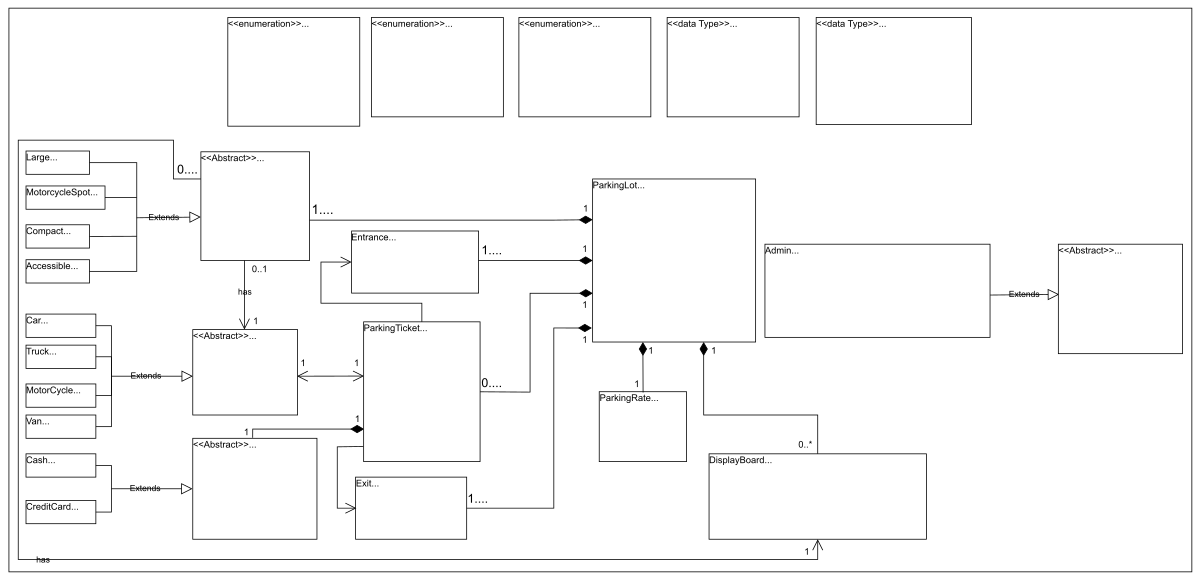
\includegraphics[width=0.5\textwidth]{Images/chapter_7/section_6722059256463360/5175699454164992.png}
 \caption{The class diagram of the parking lot system}
\end{figure}

\subsection{Design pattern}\label{-6TPwkq65gA_yWLsj7rh-}
\\
Our parking lot system employs several standard object-oriented design patterns to enhance its flexibility and maintainability:

\begin{itemize}
\item
\protect\phantomsection\label{XrQcQ4DZOKu74JZO2GRrF}
\textbf{Singleton pattern:} The \texttt{ParkingLot} class is implemented as a Singleton. This ensures that only one instance of the parking lot system exists throughout the application's life cycle, centralizing the management of all lot resources.
\item
\protect\phantomsection\label{udYBtqlm9Lox-BegAuDtv}
\textbf{Factory and Abstract Factory patterns:} Creating different types of parking spots, vehicles, or payments can leverage the Factory and Abstract Factory patterns. These patterns make it easy to introduce new types of spots, vehicles, or payment methods in the future, simply by extending the factory logic, without changing the core business logic or system structure.
\end{itemize}

\subsection{AI-powered trainer}\label{lW68H86NS2hzAuHh_BGDz}
\\
At this stage, everything should be clear. If you encounter any confusion or ambiguity, feel free to utilize the interactive AI-enabled widget below to seek clarification. This tool is designed to help you strengthen your understanding of the concepts.

\begin{figure}[htbp]
 \centering
 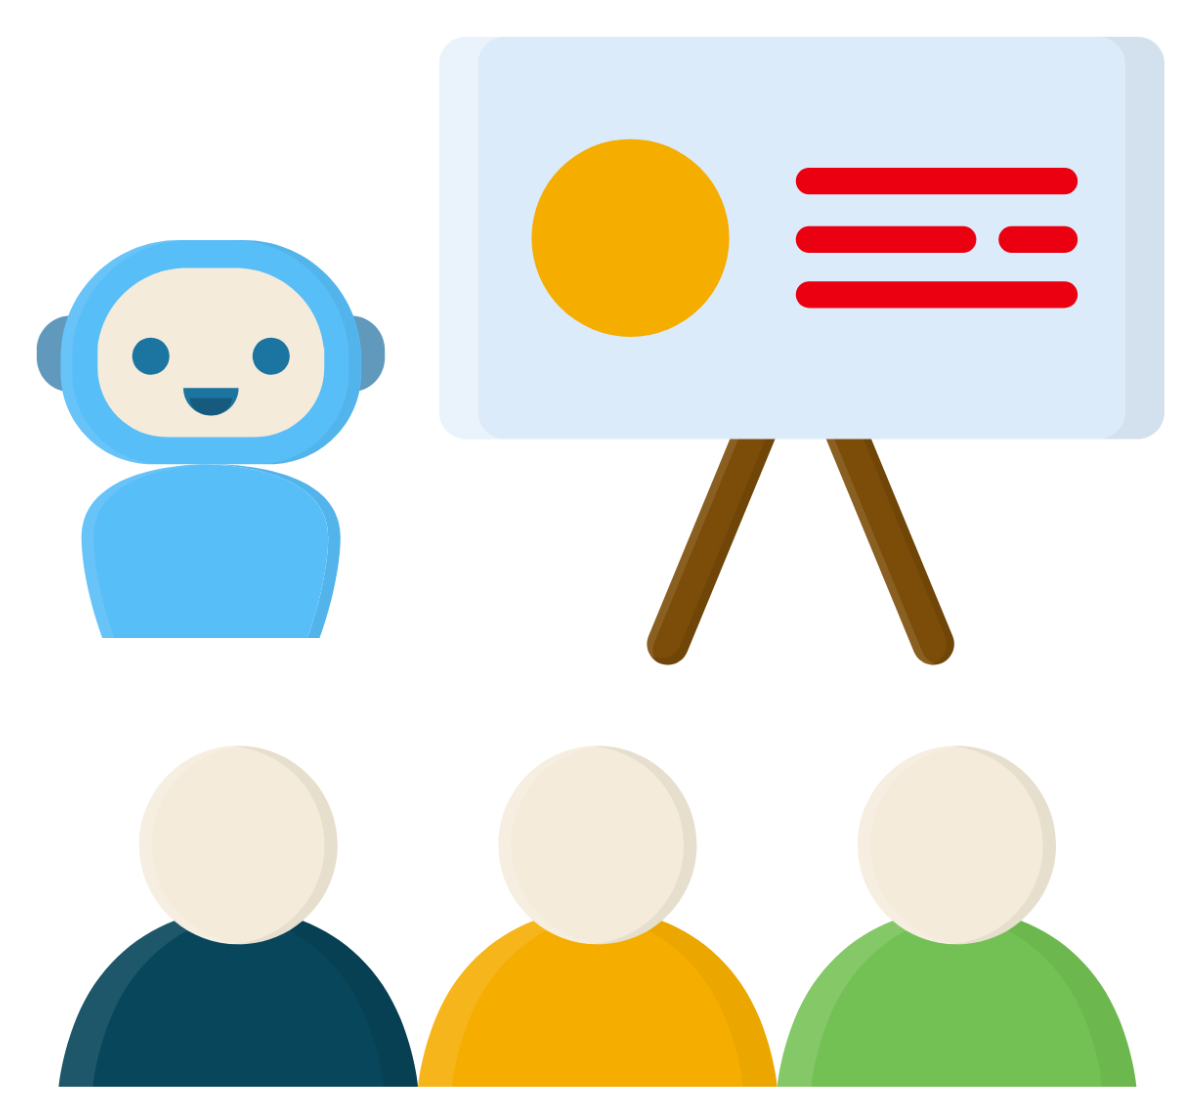
\includegraphics[width=0.15\textwidth]{Images/chapter_7/section_6722059256463360/6716918571335680.png}
 
\end{figure}

\subsection{Additional requirements}\label{_CwM6ewYcxao_UsEbd0IN}
\\
The interviewer can introduce some additional requirements in the parking lot system, or they can ask some follow-up questions. Let 's see some examples of additional requirements:
\\
\textbf{Parking floor:} The parking lot should have multiple floors where customers can park their cars. The class diagram provided below shows the relationship of \texttt{ParkingFloor} with other classes:

\begin{figure}[htbp]
 \centering
 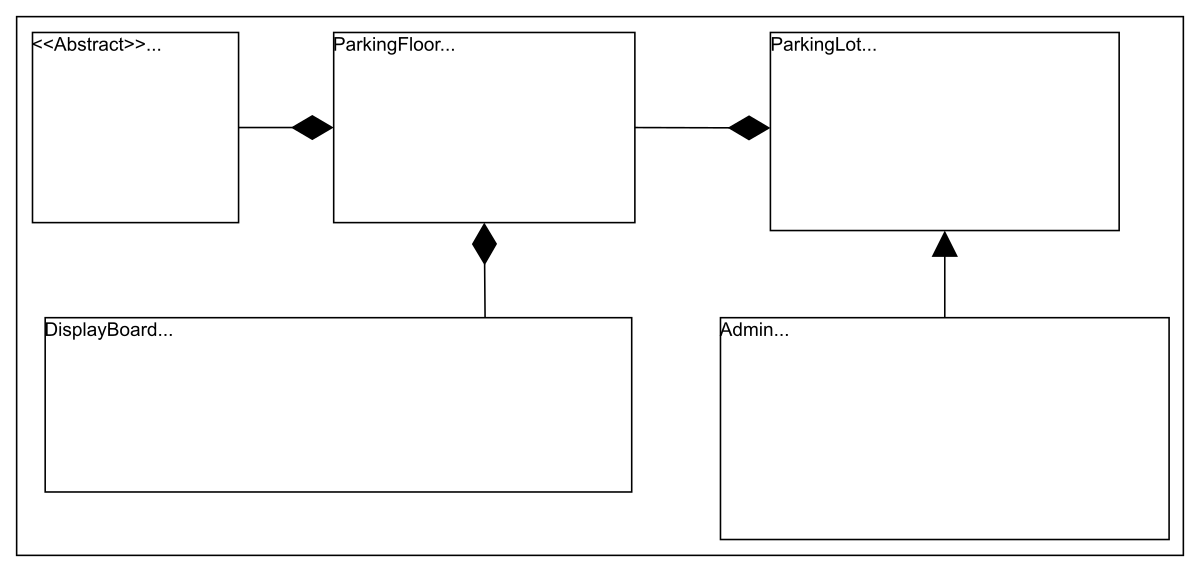
\includegraphics[width=0.5\textwidth]{Images/chapter_7/section_6722059256463360/5079841314308096.png}
 \caption{Relationship of the ParkingFloor class with other classes}
\end{figure}

\textbf{Electric:} The parking lot should have some parking spots specified for electric cars. These spots should have an electric panel through which customers can pay and charge their vehicles. The class diagram provided below shows the relationship of \texttt{Electric} and \texttt{ElectricPanel} with other classes:

\begin{figure}[htbp]
 \centering
 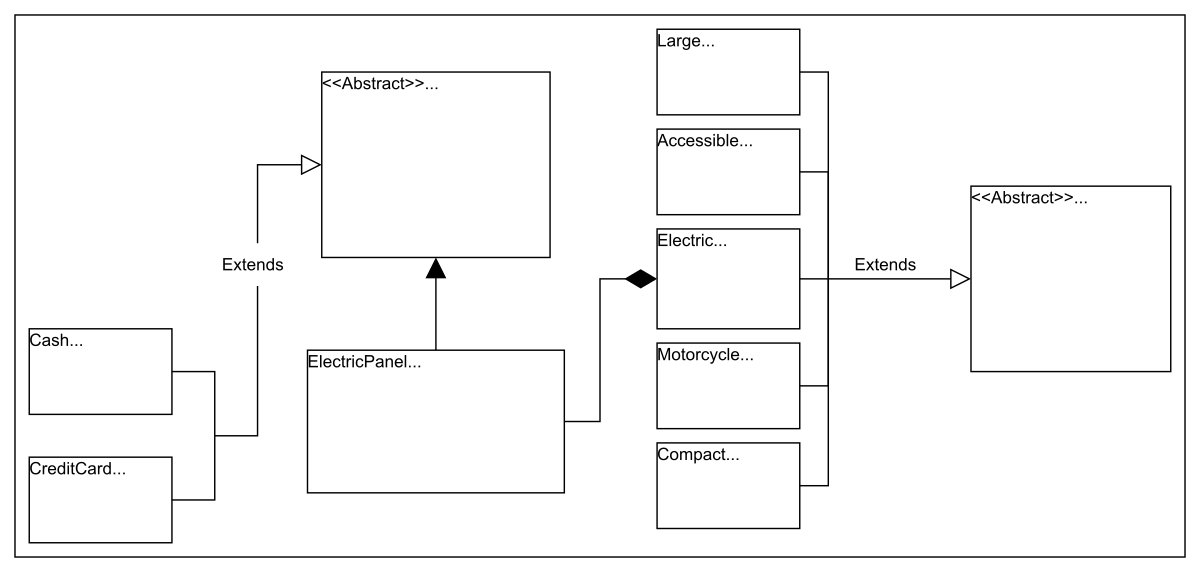
\includegraphics[width=0.5\textwidth]{Images/chapter_7/section_6722059256463360/4773499003338752.png}
 \caption{Relationship of the Electric and ElectricPanel classes with other classes}
\end{figure}

\begin{quote}
\textbf{Quiz:}
\textbf{Question 1:} Let's say that the interviewer asks you that the parking lot should assign a parking spot closest to the entrance. How do you go about solving this requirement?
\textbf{Answer:} This requirement is more about implementing this parking assignment strategy than designing it. The interviewer looks at your data structures and algorithm skills in this requirement. In this scenario,

let's say we have four entrances and would like the customer to return to the parking spot nearest to the entrance from which the customer entered the parking lot. The best approach is to implement it using a ``min heap.'' We will declare four min heaps and add all parking spots so that each entrance will have a min heap. These min heaps will store the parking spots in order of the shortest distance from the entrance. -
We will also declare the following two sets of parking spots: - A set of available parking spots - A set of reserved parking spots - We have a map of min heaps where the key is the entrance ID, and the value is a min heap. When the user calls the \_`getParkingSpot`\_ method, we get the entrance ID, which gives us the min heap for that entrance and allows us to pop the top element to get the parking spot. - We mark the parking spot as reserved and remove it from the available set. We also remove it from the min heaps of other entrances.
\end{quote}

We have completed the class diagram of the parking lot system according to the requirements. Now , let's design the sequence diagram of the parking lot system in the next lesson.

% End of section content